% Supplement to the main empirical experiment. Paths assume this is included
% from a manuscript root containing the complexity_schedule directory.
\paragraph{An initially calibrated regularization schedule.}
For the Mat\'ern-$3/2$ representation, we choose $C_0$ once using the
1963--1972 training and 1973--1977 formation-validation samples, and use
\[
\lambda_T=C_0 T^{-\widehat b_T/(\widehat b_T+1)}.
\]
Here $T$ counts historical monthly managed payoffs, and $\widehat b_T$ is
re-estimated at each January formation close together with the portfolio
coefficients. It is the negative OLS slope of log second-moment eigenvalues
on log rank, using the fixed 10\%--60\% rank band after a relative $10^{-12}$
numerical cutoff. This finite-sample estimation convention supplements the
manuscript's asymptotic rate; it does not establish its population spectral
assumption. The main-text rate corresponds to $r=1$ in the general appendix.
The grid retains all 120 previous initial-training penalties and adds 80
intermediate effective-complexity points before converting penalties to $C_0$.
Validation selects $C_0=2.265779\times10^{-6}$, available on January 31, 1978.
The constant remains unchanged during all 47 subsequent annual refits.

Selected effective complexity rises from 36.681 in 1978 to 91.776 in 2024;
regularization falls from $1.15864\times10^{-7}$ to $4.67964\times10^{-8}$.
Annual spectral estimates range from 1.3309 to 1.4323. The 564 selected
OOS monthly payoffs have an annualized Sharpe of 3.561. This remains an
exceptionally strong gross backtest, subject to the same complete-case payoff
selection, retrospective characteristic dictionary, current-snapshot and
execution assumptions as the main experiment; trading and borrowing costs
are not subtracted.

Each annual curve evaluates only its twelve subsequent payoffs, from February
through the following January. Annual Sharpe estimates are therefore noisy.
Loss is the unscaled held-out mean of $(1-R^p)^2$, with no test-period ridge
penalty and no wealth-plot scaling. Neither the OOS loss nor OOS Sharpe selects
$C_0$, the spectral rank band, or the annual coefficients. Changes in estimated
$b$ could make the plug-in regularization path locally nonmonotonic, although
no annual increases occur in this sample. No curve shape is imposed.

\begin{figure}[htbp]\centering
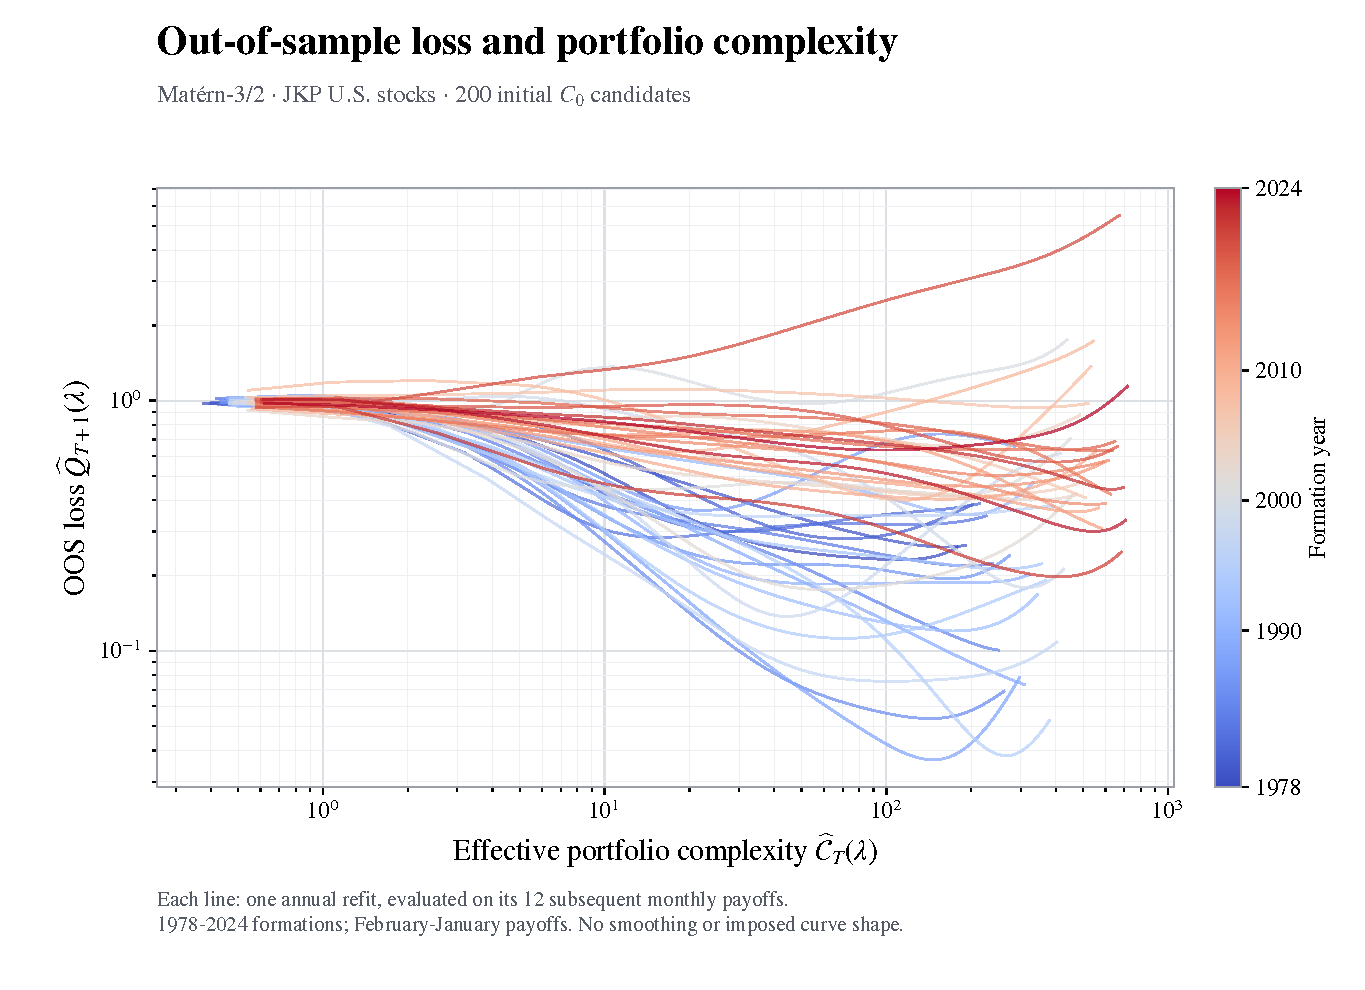
\includegraphics[width=\linewidth]{complexity_schedule/fig01_oos_loss.pdf}
\caption{Next-year OOS quadratic loss against effective complexity for every
annual Mat\'ern refit, 1978--2024. Colors indicate formation years.}
\label{fig:schedule-oos-loss}\end{figure}
\begin{figure}[htbp]\centering
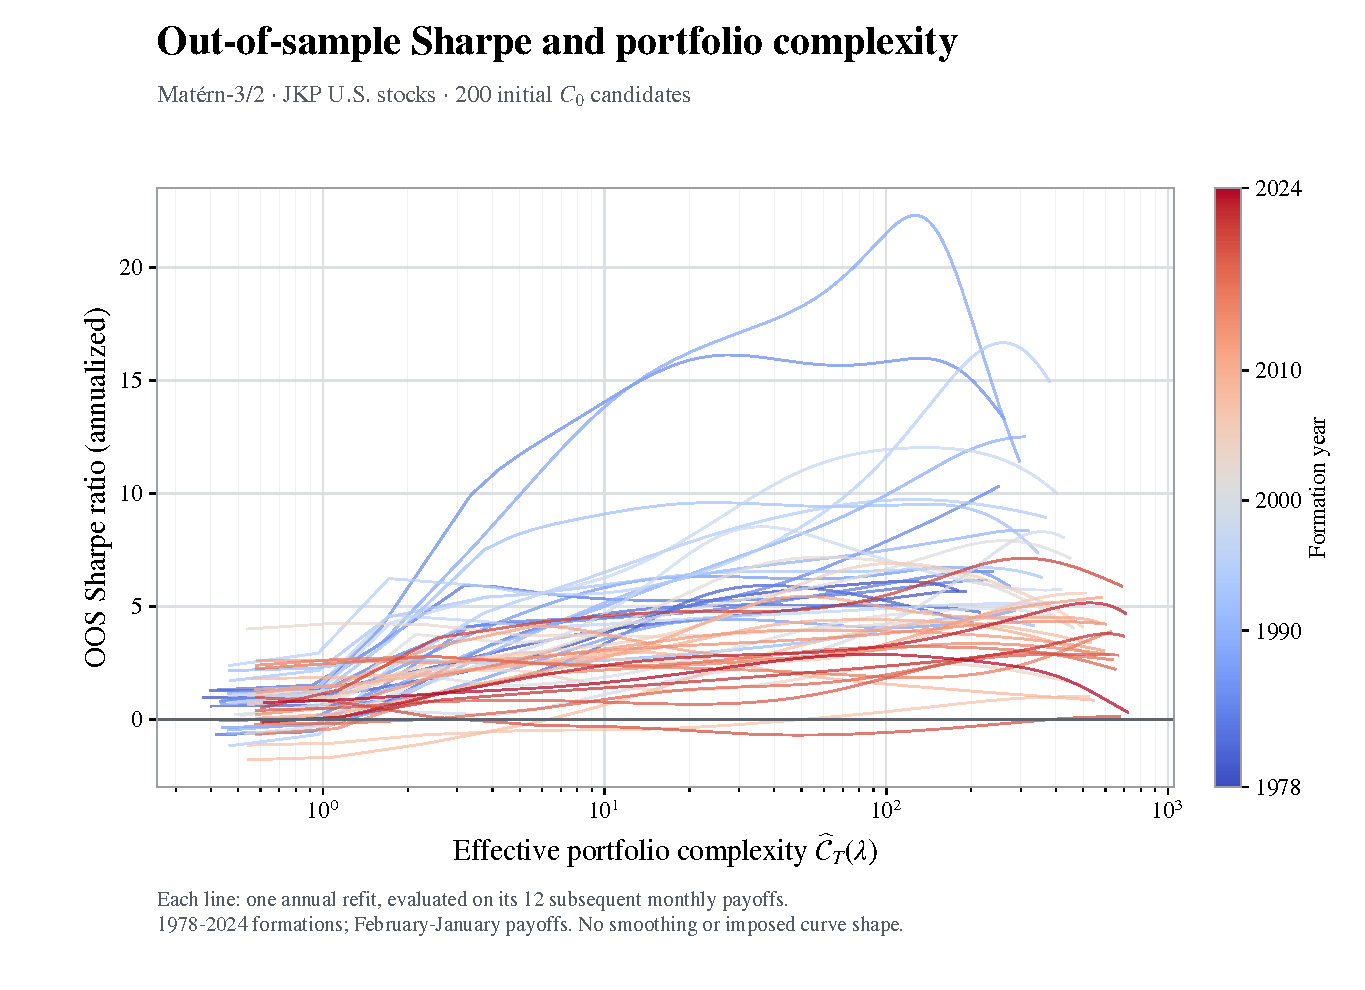
\includegraphics[width=\linewidth]{complexity_schedule/fig02_oos_sharpe.pdf}
\caption{Annualized Sharpe against effective complexity, computed separately
from each twelve-month OOS window.}
\label{fig:schedule-oos-sharpe}\end{figure}
\begin{figure}[htbp]\centering
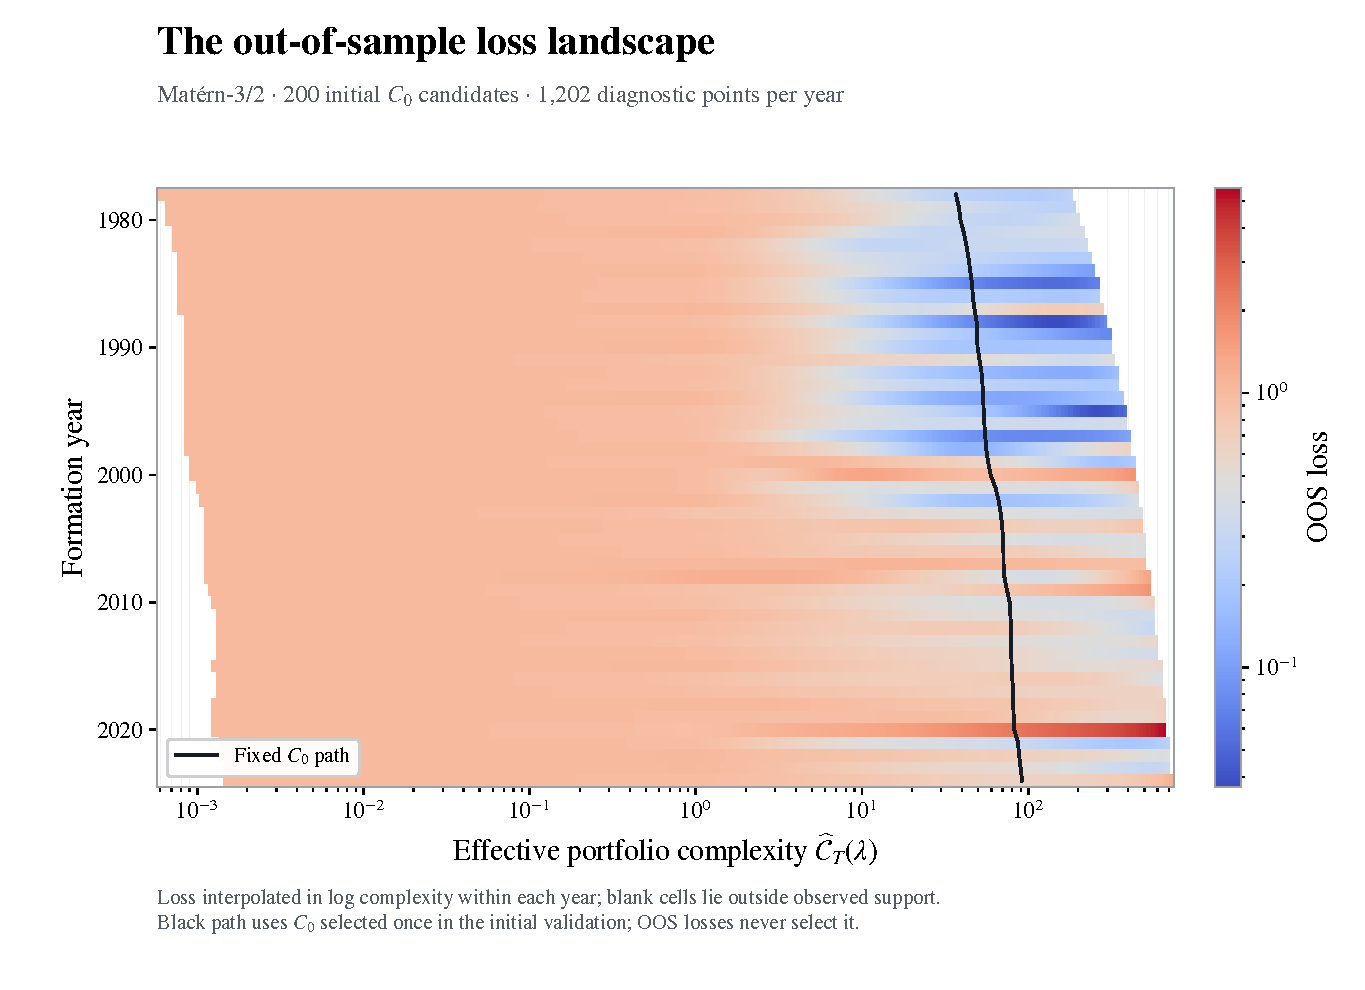
\includegraphics[width=\linewidth]{complexity_schedule/fig03_oos_loss_heatmap.pdf}
\caption{OOS loss by formation year and effective complexity. Interpolation
is confined to each year's observed complexity support. The black line is the
path implied by the initially selected, fixed $C_0$.}
\label{fig:schedule-heatmap}\end{figure}
\begin{figure}[htbp]\centering
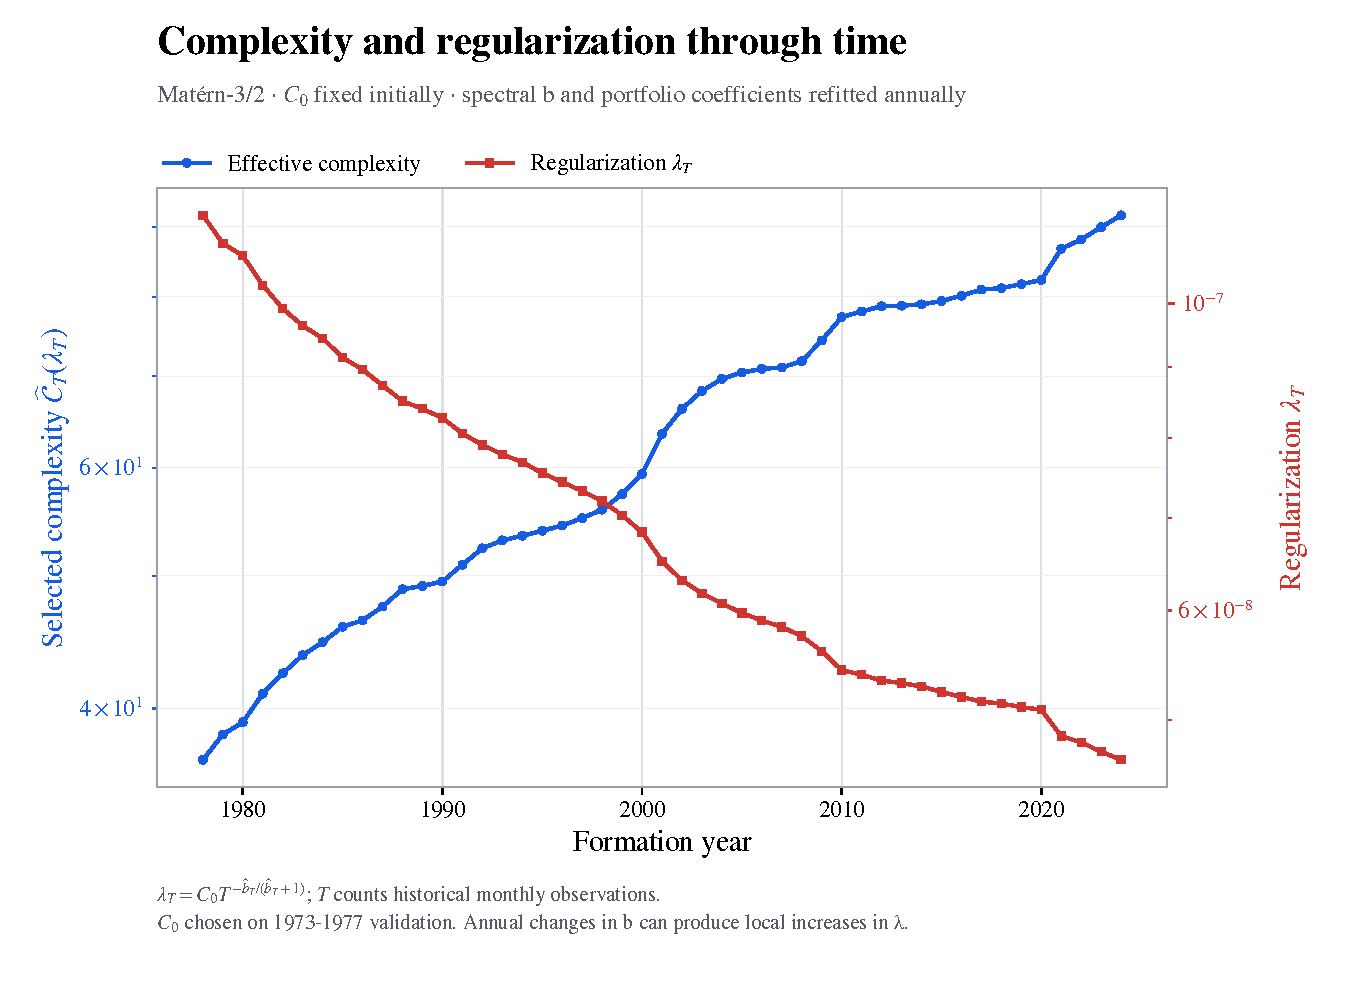
\includegraphics[width=\linewidth]{complexity_schedule/fig04_complexity_regularization.pdf}
\caption{Effective complexity and regularization implied by a fixed initial
$C_0$ and annually updated historical spectral estimates.}
\label{fig:schedule-path}\end{figure}
